% ==========================================================================
%  Computational set-up and Edney type IV shock structure (detailed)
%  (a) computational domain and boundary conditions,
%  (b) close-up of the Edney type IV interaction (dashed box in (a)).
%
%  Standalone LaTeX file.  On Overleaf: New Project > Blank Project, replace
%  the whole of main.tex with this file (or upload it and set it as the main
%  document), compiler pdfLaTeX.  To use the figure in a paper, compile this
%  file and include the PDF with \includegraphics.
%
%  Generated by make_tikz.py.  Coordinates in mm, origin at the cylinder
%  centre, x downstream, y up; phi measured from the stagnation point.
%  Shock positions: no-field shock trace (data/bow_shock_no_field.csv) and its
%  Billig-type far-field fit.
%  Case: M_inf = 8.03, beta = 18.1 deg -> theta = 12.49 deg, M_2 = 5.252;
%        transmitted shock -26.1 deg -> jet direction -15.1 deg,
%        M_jet = 2.41, jet width 4.5 mm  (oblique-shock relations, gamma = 1.4).
%        R = 38.1 mm, inlet radius 150 mm, outlets at phi = +/-65 deg,
%        no-slip wall |phi| <= 45 deg, slip wall beyond, inlet split phi = -12.25 deg.
%  Jet shock cells and expansion fans are schematic (drawn steeper than
%  the jet Mach angle for legibility).
% ==========================================================================
\documentclass[border=1.5pt]{standalone}
% ---- fonts: Helvetica text; sans-serif math (newtxsf) when available
\usepackage[T1]{fontenc}
\usepackage[scaled=0.92]{helvet}
\renewcommand{\familydefault}{\sfdefault}
\IfFileExists{newtxsf.sty}{\usepackage{newtxsf}}{}
\usepackage{tikz}
\usetikzlibrary{arrows.meta}

% ---- colours
\definecolor{ink}{HTML}{111111}
\definecolor{shockgrey}{HTML}{4A4A4A}
\definecolor{dimgrey}{HTML}{8A8A8A}
\definecolor{leadergrey}{HTML}{A0A0A0}
\definecolor{bodygrey}{HTML}{E4E4E4}
\definecolor{freeblue}{HTML}{1A5FA8}
\definecolor{postgreen}{HTML}{0E8A62}
\definecolor{slipochre}{HTML}{B06A10}
\definecolor{jetfill}{HTML}{FBEBD3}
\definecolor{jetedge}{HTML}{8C5A14}

% ---- styles
\tikzset{
  lbl/.style={font=\sffamily\footnotesize, text=ink, inner sep=1.2pt, align=center},
  small/.style={font=\sffamily\scriptsize},
  region/.style={font=\sffamily\footnotesize, text=dimgrey, inner sep=1pt},
  leader/.style={draw=leadergrey, line width=0.35pt},
  freeinlet/.style={draw=freeblue, line width=1.5pt},
  postinlet/.style={draw=postgreen, line width=1.5pt},
  outlet/.style={draw=dimgrey, line width=1.1pt, dash pattern=on 3.2pt off 2pt, line cap=butt},
  noslip/.style={draw=ink, line width=1.7pt},
  slip/.style={draw=slipochre, line width=1.7pt, dash pattern=on 2pt off 1.1pt, line cap=butt},
  shockA/.style={draw=shockgrey, line width=0.7pt},
  shockB/.style={draw=ink, line width=1.15pt},
  jetshock/.style={draw=ink, line width=1.0pt},
  shear/.style={draw=ink, line width=0.7pt, dash pattern=on 2.4pt off 1.4pt, line cap=butt},
  cellshock/.style={draw=jetedge, line width=0.45pt},
  fan/.style={draw=jetedge, line width=0.35pt, dash pattern=on 1.1pt off 0.9pt, line cap=butt},
  flow/.style={line width=0.9pt, -{Stealth[length=2.6mm, width=1.9mm]}},
  jetflow/.style={draw=ink, line width=0.7pt, -{Stealth[length=1.9mm, width=1.4mm]}},
  dim/.style={draw=dimgrey, line width=0.45pt,
              {Stealth[length=1.6mm, width=1.1mm]}-{Stealth[length=1.6mm, width=1.1mm]}},
  triple/.style={circle, fill=ink, inner sep=0pt, minimum size=1.5mm},
  dot/.style={circle, fill=leadergrey, inner sep=0pt, minimum size=0.9mm},
}

\begin{document}
\sffamily\footnotesize
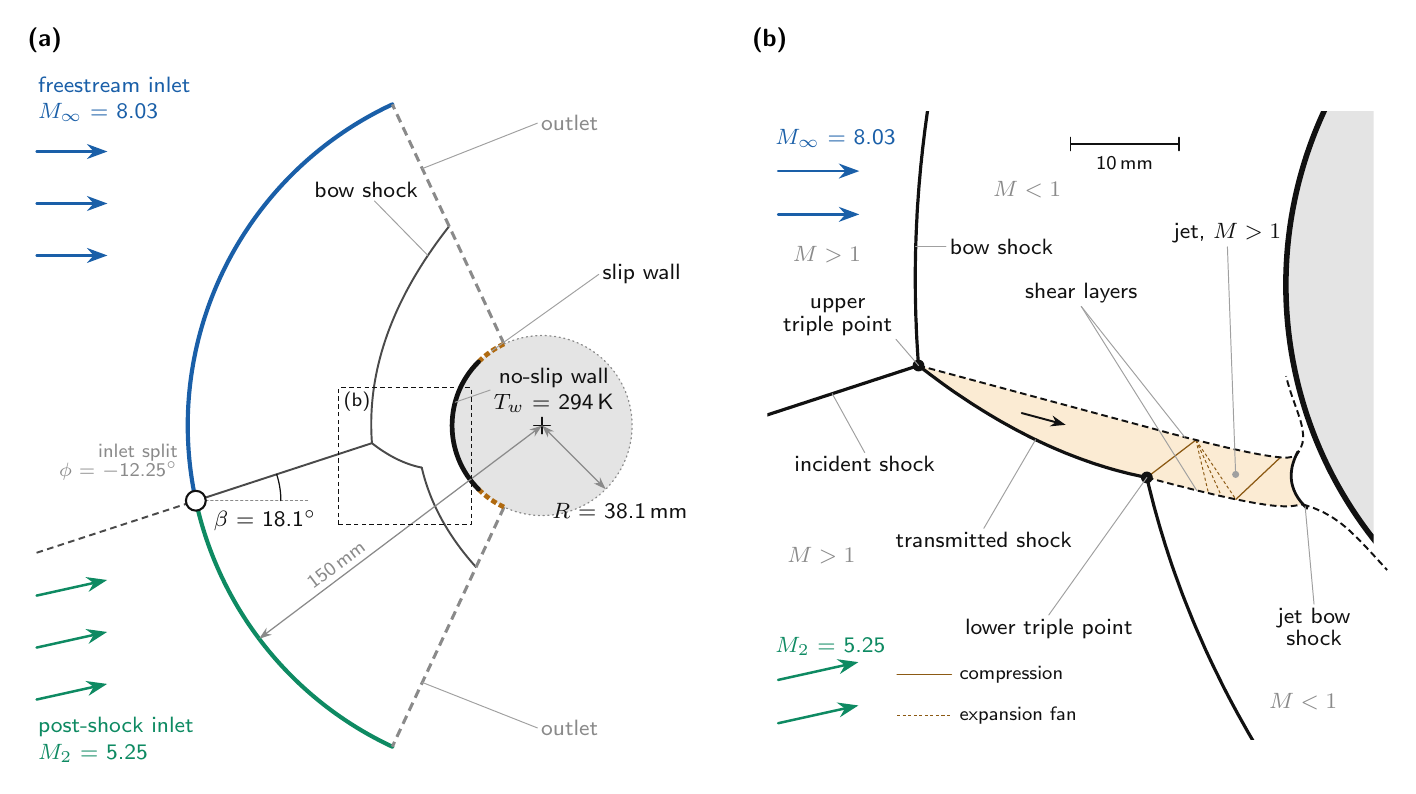
\begin{tikzpicture}[x=1mm, y=1mm, line cap=round, line join=round]

% ==========================================================================
%  (a)  computational domain              scale 1 : 3.33
% ==========================================================================
\begin{scope}[shift={(65.4,45.6)}, x=0.3mm, y=0.3mm]

  % cylinder (dotted outline where it lies outside the domain)
  \fill[bodygrey] (0,0) circle[radius=38.1];
  \draw[dimgrey, line width=0.45pt, dash pattern=on 0.4pt off 1.3pt]
    (115.0:38.1) arc[start angle=115.0, end angle=-115.0, radius=38.1];

  % shock system, clipped to the domain
  \begin{scope}
    \clip (115.0:150.0) arc[start angle=115.0, end angle=245.0, radius=150.0]
      -- (245.0:38.1) arc[start angle=245.0, end angle=115.0, radius=38.1] -- cycle;
    \draw[shockA]
      (-72.03,-7.46) -- (-72.18,-5.05) -- (-72.28,-2.64) -- (-72.33,-0.23) --
      (-72.32,2.18) -- (-72.25,4.59) -- (-72.13,7) -- (-71.96,9.41) -- (-71.73,11.82) --
      (-71.45,14.23) -- (-71.11,16.64) -- (-70.72,19.05) -- (-70.27,21.46) --
      (-69.77,23.86) -- (-69.21,26.27) -- (-68.6,28.68) -- (-67.94,31.09) -- (-67.22,33.5) --
      (-66.44,35.91) -- (-65.62,38.32) -- (-64.73,40.73) -- (-63.79,43.14) --
      (-62.8,45.55) -- (-61.76,47.96) -- (-60.66,50.37) -- (-59.5,52.78) -- (-58.29,55.19) --
      (-57.03,57.6) -- (-55.71,60.01) -- (-54.34,62.42) -- (-52.91,64.83) --
      (-51.43,67.24) -- (-49.9,69.64) -- (-48.31,72.05) -- (-46.66,74.46) --
      (-44.97,76.87) -- (-43.22,79.28) -- (-41.41,81.69) -- (-39.55,84.1) --
      (-37.64,86.51) -- (-35.68,88.92) -- (-33.66,91.33) -- (-31.58,93.74) --
      (-29.45,96.15) -- (-27.27,98.56) -- (-25.04,100.97) -- (-22.75,103.38) --
      (-20.41,105.79) -- (-18.02,108.2) -- (-15.57,110.61) -- (-13.07,113.02) --
      (-10.51,115.42) -- (-7.9,117.83) -- (-5.24,120.24) -- (-2.53,122.65) --
      (0.24,125.06) -- (3.06,127.47) -- (5.93,129.88) -- (8.86,132.29) -- (11.83,134.7) --
      (14.86,137.11) -- (17.95,139.52) -- (21.08,141.93) -- (24.27,144.34) --
      (27.51,146.75) -- (30.8,149.16) -- (34.15,151.57) -- (37.55,153.98) -- (41,156.39) --
      (44.5,158.8) -- (46.27,160);
    \draw[shockA]
      (-50.94,-17.8) -- (-50.38,-20.09) -- (-49.75,-22.36) -- (-49.05,-24.62) --
      (-48.29,-26.86) -- (-47.46,-29.09) -- (-46.57,-31.3) -- (-45.61,-33.5) --
      (-44.58,-35.68) -- (-43.49,-37.85) -- (-42.34,-40.01) -- (-41.12,-42.15) --
      (-39.83,-44.28) -- (-38.48,-46.39) -- (-37.06,-48.49) -- (-35.58,-50.57) --
      (-34.04,-52.64) -- (-32.42,-54.7) -- (-30.75,-56.74) -- (-29.01,-58.76) --
      (-27.2,-60.77) -- (-25.33,-62.77) -- (-23.4,-64.75) -- (-21.4,-66.72) --
      (-19.34,-68.68) -- (-17.21,-70.62) -- (-15.02,-72.55) -- (-12.77,-74.46) --
      (-10.45,-76.36) -- (-8.07,-78.24) -- (-5.63,-80.11) -- (-3.12,-81.97) --
      (-0.55,-83.81) -- (2.08,-85.64) -- (4.77,-87.45) -- (7.53,-89.25) -- (10.35,-91.04) --
      (13.23,-92.82) -- (16.17,-94.58) -- (19.17,-96.32) -- (22.24,-98.05) --
      (25.36,-99.77) -- (28.55,-101.48) -- (31.8,-103.17) -- (35.1,-104.85) --
      (38.47,-106.52) -- (41.9,-108.17) -- (45.38,-109.81) -- (48.93,-111.43) --
      (52.54,-113.05) -- (56.2,-114.65) -- (59.92,-116.23) -- (63.71,-117.81) --
      (67.55,-119.37) -- (71.44,-120.92) -- (75.4,-122.45) -- (79.41,-123.97) --
      (83.48,-125.48) -- (87.61,-126.98) -- (91.79,-128.47) -- (96.03,-129.94) --
      (100.33,-131.4) -- (104.68,-132.85) -- (109.09,-134.28) -- (113.55,-135.71) --
      (118.06,-137.12) -- (122.64,-138.52) -- (127.26,-139.9) -- (131.94,-141.28) --
      (136.67,-142.64) -- (139.06,-143.32);
    \draw[shockA]
      (-72.03,-7.46) -- (-70.95,-8.29) -- (-69.87,-9.09) -- (-68.79,-9.86) --
      (-67.7,-10.59) -- (-66.62,-11.29) -- (-65.54,-11.96) -- (-64.46,-12.6) --
      (-63.38,-13.2) -- (-62.3,-13.77) -- (-61.22,-14.31) -- (-60.13,-14.82) --
      (-59.05,-15.29) -- (-57.97,-15.73) -- (-56.89,-16.14) -- (-55.81,-16.52) --
      (-54.73,-16.86) -- (-53.65,-17.17) -- (-52.56,-17.45) -- (-51.48,-17.69) --
      (-50.94,-17.8);
    \draw[shockA] (-146.58,-31.83) -- (-72.03,-7.46);
  \end{scope}

  % imposed oblique shock upstream of the inlet
  \draw[shockA, dash pattern=on 2.4pt off 1.6pt, line cap=butt] (-214,-53.86) -- (-146.58,-31.83);

  % inlets and outlets
  \draw[freeinlet] (192.25:150.0) arc[start angle=192.25, end angle=115.0, radius=150.0];
  \draw[postinlet] (245.0:150.0) arc[start angle=245.0, end angle=192.25, radius=150.0];
  \draw[outlet] (115.0:38.1) -- (115.0:150.0);
  \draw[outlet] (245.0:38.1) -- (245.0:150.0);

  % walls: no-slip for |phi| <= 45 deg, slip for 45 < |phi| <= 65 deg
  \draw[slip]   (115.0:38.1) arc[start angle=115.0, end angle=135.0, radius=38.1];
  \draw[slip]   (225.0:38.1) arc[start angle=225.0, end angle=245.0, radius=38.1];
  \draw[noslip] (135.0:38.1) arc[start angle=135.0, end angle=225.0, radius=38.1];
  \draw[ink, line width=0.5pt] (-3.5,0) -- (3.5,0) (0,-3.5) -- (0,3.5);

  % inlet split and shock angle
  \draw[dimgrey, line width=0.4pt, dash pattern=on 0.8pt off 1pt] (-146.58,-31.83) -- ++(48,0);
  \draw[ink, line width=0.45pt] (-110.58,-31.83) arc[start angle=0, end angle=18.100000000000005, radius=36];
  \node[lbl, anchor=north west] at (-140.58,-34.33) {$\beta$ = 18.1$^\circ$};
  \filldraw[fill=white, draw=ink, line width=0.75pt] (-146.58,-31.83) circle[radius=4.2];
  \node[lbl, small, text=dimgrey, anchor=south east, align=right] at (-152.58,-24.83)
    {inlet split\\[-0.3ex]$\phi$ = $-$12.25$^\circ$};

  % inflow
  \foreach \yy in {116, 94, 72} {\draw[flow, freeblue] (-214,\yy) -- ++(30,0);}
  \foreach \yy in {-72, -94, -116} {\draw[flow, postgreen] (-214,\yy) -- ++(12.49:30.6);}
  \node[lbl, text=freeblue, anchor=south west, align=left] at (-215,127)
    {freestream inlet\\$M_\infty$ = 8.03};
  \node[lbl, text=postgreen, anchor=north west, align=left] at (-215,-122)
    {post-shock inlet\\$M_2$ = 5.25};

  % boundary labels
  \node[lbl] (ns) at (5,15) {no-slip wall\\$T_w$ = 294\,K};
  \draw[leader] (ns.west) -- (-36.8,9.86);
  \node[lbl, anchor=west] (sw) at (24,64) {slip wall};
  \draw[leader] (sw.west) -- (-21.31,31.59);
  \node[lbl, text=dimgrey, anchor=west] (o1) at (-2,128) {outlet};
  \draw[leader] (o1.west) -- (115.0:120);
  \node[lbl, text=dimgrey, anchor=west] (o2) at (-2,-128) {outlet};
  \draw[leader] (o2.west) -- (245.0:120);
  \node[lbl, anchor=west] (bs) at (-98,100) {bow shock};
  \draw[leader] ([xshift=-6mm]bs.south east) -- (-48.34,72);

  % dimensions
  \draw[dim] (0,0) -- (-45:38.1);
  \node[lbl, anchor=north] at (32.94,-31.44) {$R$ = 38.1\,mm};
  \draw[dim] (0,0) -- (217.0:150.0);
  \node[lbl, small, text=dimgrey, rotate=37.00] at (-87.17,-58.8) {150\,mm};

  % window shown in (b)
  \draw[ink, line width=0.4pt, dash pattern=on 1.6pt off 1.2pt, line cap=butt]
    (-86,-42) rectangle (-30,16);
  \node[lbl, small, anchor=north west, inner sep=1.5pt] at (-86,16) {(b)};
\end{scope}

% ==========================================================================
%  (b)  type IV interaction               scale 1.375 : 1
% ==========================================================================
\begin{scope}[shift={(212.25,63.48)}, x=1.3750mm, y=1.3750mm]
  \begin{scope}
    \clip (-86,-42) rectangle (-30,16);

    % body and wall
    \fill[bodygrey] (0,0) circle[radius=38.1];
    \draw[noslip, line width=2pt] (135.0:38.1) arc[start angle=135.0, end angle=225.0, radius=38.1];
    \draw[slip, line width=2pt] (115.0:38.1) arc[start angle=115.0, end angle=135.0, radius=38.1];
    \draw[slip, line width=2pt] (225.0:38.1) arc[start angle=225.0, end angle=245.0, radius=38.1];

    % supersonic jet: transmitted shock, shear layers and jet bow shock
    \fill[jetfill]
      (-72.03,-7.46) -- (-49.67,-13.49) -- (-49.45,-13.54) -- (-49.24,-13.6) --
      (-49.04,-13.66) -- (-48.83,-13.71) -- (-48.63,-13.77) -- (-48.42,-13.82) --
      (-48.22,-13.87) -- (-48.02,-13.92) -- (-47.83,-13.98) -- (-47.63,-14.03) --
      (-47.44,-14.08) -- (-47.24,-14.13) -- (-47.05,-14.18) -- (-46.87,-14.22) --
      (-46.68,-14.27) -- (-46.49,-14.32) -- (-46.31,-14.36) -- (-46.13,-14.41) --
      (-45.95,-14.46) -- (-45.77,-14.5) -- (-45.6,-14.54) -- (-45.42,-14.59) --
      (-45.25,-14.63) -- (-45.08,-14.67) -- (-44.91,-14.71) -- (-44.74,-14.75) --
      (-44.58,-14.79) -- (-44.42,-14.83) -- (-44.25,-14.87) -- (-44.09,-14.91) --
      (-43.94,-14.94) -- (-43.78,-14.98) -- (-43.63,-15.02) -- (-43.47,-15.05) --
      (-43.32,-15.09) -- (-43.17,-15.12) -- (-43.03,-15.15) -- (-42.88,-15.19) --
      (-42.74,-15.22) -- (-42.6,-15.25) -- (-42.46,-15.28) -- (-42.32,-15.31) --
      (-42.18,-15.34) -- (-42.05,-15.37) -- (-41.92,-15.39) -- (-41.79,-15.42) --
      (-41.66,-15.45) -- (-41.53,-15.47) -- (-41.4,-15.5) -- (-41.28,-15.52) --
      (-41.16,-15.55) -- (-41.04,-15.57) -- (-40.92,-15.59) -- (-40.81,-15.61) --
      (-40.69,-15.64) -- (-40.58,-15.66) -- (-40.47,-15.68) -- (-40.37,-15.7) --
      (-40.26,-15.71) -- (-40.16,-15.73) -- (-40.05,-15.75) -- (-39.95,-15.77) --
      (-39.86,-15.78) -- (-39.76,-15.8) -- (-39.67,-15.81) -- (-39.57,-15.83) --
      (-39.48,-15.84) -- (-39.4,-15.85) -- (-39.31,-15.86) -- (-39.23,-15.87) --
      (-39.15,-15.88) -- (-39.07,-15.89) -- (-38.99,-15.9) -- (-38.91,-15.91) --
      (-38.84,-15.92) -- (-38.77,-15.93) -- (-38.7,-15.93) -- (-38.64,-15.94) --
      (-38.57,-15.95) -- (-38.51,-15.95) -- (-38.45,-15.96) -- (-38.4,-15.96) --
      (-38.35,-15.96) -- (-38.29,-15.96) -- (-38.25,-15.97) -- (-38.2,-15.97) --
      (-38.16,-15.97) -- (-38.12,-15.97) -- (-38.08,-15.97) -- (-38.05,-15.97) --
      (-38.02,-15.97) -- (-37.99,-15.97) -- (-37.97,-15.97) -- (-37.95,-15.97) --
      (-37.94,-15.96) -- (-37.93,-15.96) -- (-37.92,-15.96) -- (-37.92,-15.96) --
      (-37.92,-15.96) -- (-37.31,-16.11) -- (-37.47,-16.61) -- (-37.58,-17.11) --
      (-37.61,-17.59) -- (-37.59,-18.07) -- (-37.5,-18.53) -- (-37.35,-18.99) --
      (-37.13,-19.43) -- (-36.85,-19.87) -- (-36.51,-20.29) -- (-37.27,-20.41) --
      (-37.36,-20.42) -- (-37.44,-20.43) -- (-37.53,-20.44) -- (-37.61,-20.45) --
      (-37.7,-20.46) -- (-37.78,-20.46) -- (-37.87,-20.46) -- (-37.95,-20.47) --
      (-38.03,-20.47) -- (-38.12,-20.47) -- (-38.2,-20.47) -- (-38.29,-20.46) --
      (-38.37,-20.46) -- (-38.46,-20.46) -- (-38.54,-20.45) -- (-38.63,-20.45) --
      (-38.72,-20.44) -- (-38.81,-20.44) -- (-38.9,-20.43) -- (-38.99,-20.42) --
      (-39.08,-20.42) -- (-39.18,-20.41) -- (-39.27,-20.4) -- (-39.37,-20.39) --
      (-39.47,-20.38) -- (-39.56,-20.36) -- (-39.66,-20.35) -- (-39.77,-20.34) --
      (-39.87,-20.33) -- (-39.97,-20.31) -- (-40.08,-20.3) -- (-40.18,-20.28) --
      (-40.29,-20.26) -- (-40.4,-20.25) -- (-40.51,-20.23) -- (-40.62,-20.21) --
      (-40.74,-20.19) -- (-40.85,-20.18) -- (-40.97,-20.16) -- (-41.09,-20.13) --
      (-41.21,-20.11) -- (-41.33,-20.09) -- (-41.45,-20.07) -- (-41.58,-20.05) --
      (-41.7,-20.02) -- (-41.83,-20) -- (-41.96,-19.97) -- (-42.09,-19.95) --
      (-42.22,-19.92) -- (-42.36,-19.89) -- (-42.49,-19.87) -- (-42.63,-19.84) --
      (-42.77,-19.81) -- (-42.91,-19.78) -- (-43.05,-19.75) -- (-43.19,-19.72) --
      (-43.34,-19.69) -- (-43.48,-19.66) -- (-43.63,-19.62) -- (-43.78,-19.59) --
      (-43.93,-19.56) -- (-44.09,-19.52) -- (-44.24,-19.49) -- (-44.4,-19.45) --
      (-44.56,-19.42) -- (-44.72,-19.38) -- (-44.88,-19.34) -- (-45.04,-19.3) --
      (-45.21,-19.26) -- (-45.37,-19.23) -- (-45.54,-19.18) -- (-45.71,-19.14) --
      (-45.89,-19.1) -- (-46.06,-19.06) -- (-46.23,-19.02) -- (-46.41,-18.97) --
      (-46.59,-18.93) -- (-46.77,-18.89) -- (-46.95,-18.84) -- (-47.13,-18.79) --
      (-47.32,-18.75) -- (-47.51,-18.7) -- (-47.69,-18.65) -- (-47.88,-18.6) --
      (-48.08,-18.56) -- (-48.27,-18.51) -- (-48.47,-18.46) -- (-48.66,-18.4) --
      (-48.86,-18.35) -- (-49.06,-18.3) -- (-49.26,-18.25) -- (-49.47,-18.19) --
      (-49.67,-18.14) -- (-49.88,-18.08) -- (-50.09,-18.03) -- (-50.3,-17.97) --
      (-50.51,-17.92) -- (-50.73,-17.86) -- (-50.94,-17.8) -- (-52.02,-17.57) --
      (-53.11,-17.31) -- (-54.19,-17.02) -- (-55.27,-16.69) -- (-56.35,-16.33) --
      (-57.43,-15.94) -- (-58.51,-15.52) -- (-59.59,-15.06) -- (-60.67,-14.57) --
      (-61.76,-14.05) -- (-62.84,-13.49) -- (-63.92,-12.9) -- (-65,-12.28) --
      (-66.08,-11.63) -- (-67.16,-10.95) -- (-68.24,-10.23) -- (-69.33,-9.48) --
      (-70.41,-8.69) -- (-71.49,-7.88) -- (-72.03,-7.46) -- cycle;

    % bow shock above and below the interaction, incident shock
    \draw[shockB]
      (-72.03,-7.46) -- (-72.05,-7.13) -- (-72.08,-6.8) -- (-72.1,-6.47) -- (-72.12,-6.13) --
      (-72.14,-5.8) -- (-72.16,-5.47) -- (-72.18,-5.14) -- (-72.2,-4.81) -- (-72.21,-4.48) --
      (-72.23,-4.15) -- (-72.24,-3.82) -- (-72.25,-3.49) -- (-72.27,-3.16) --
      (-72.28,-2.82) -- (-72.29,-2.49) -- (-72.3,-2.16) -- (-72.3,-1.83) -- (-72.31,-1.5) --
      (-72.32,-1.17) -- (-72.32,-0.84) -- (-72.32,-0.51) -- (-72.33,-0.18) --
      (-72.33,0.15) -- (-72.33,0.49) -- (-72.33,0.82) -- (-72.33,1.15) -- (-72.33,1.48) --
      (-72.32,1.81) -- (-72.32,2.14) -- (-72.31,2.47) -- (-72.31,2.8) -- (-72.3,3.13) --
      (-72.29,3.46) -- (-72.28,3.8) -- (-72.27,4.13) -- (-72.26,4.46) -- (-72.24,4.79) --
      (-72.23,5.12) -- (-72.22,5.45) -- (-72.2,5.78) -- (-72.18,6.11) -- (-72.17,6.44) --
      (-72.15,6.77) -- (-72.13,7.11) -- (-72.11,7.44) -- (-72.08,7.77) -- (-72.06,8.1) --
      (-72.04,8.43) -- (-72.01,8.76) -- (-71.99,9.09) -- (-71.96,9.42) -- (-71.93,9.75) --
      (-71.9,10.08) -- (-71.87,10.42) -- (-71.84,10.75) -- (-71.81,11.08) --
      (-71.77,11.41) -- (-71.74,11.74) -- (-71.7,12.07) -- (-71.67,12.4) -- (-71.63,12.73) --
      (-71.59,13.06) -- (-71.55,13.39) -- (-71.51,13.73) -- (-71.47,14.06) --
      (-71.43,14.39) -- (-71.38,14.72) -- (-71.34,15.05) -- (-71.29,15.38) --
      (-71.25,15.71) -- (-71.2,16.04) -- (-71.15,16.37) -- (-71.1,16.7) -- (-71.05,17.04) --
      (-71,17.37) -- (-70.94,17.7) -- (-70.89,18.03) -- (-70.84,18.36) -- (-70.78,18.69) --
      (-70.72,19.02) -- (-70.66,19.35) -- (-70.61,19.68) -- (-70.54,20.01) --
      (-70.48,20.35) -- (-70.42,20.68) -- (-70.36,21.01) -- (-70.29,21.34) --
      (-70.23,21.67) -- (-70.16,22);
    \draw[shockB]
      (-50.94,-17.8) -- (-50.73,-18.7) -- (-50.5,-19.6) -- (-50.27,-20.5) --
      (-50.02,-21.39) -- (-49.77,-22.28) -- (-49.5,-23.17) -- (-49.23,-24.06) --
      (-48.94,-24.95) -- (-48.65,-25.83) -- (-48.34,-26.71) -- (-48.02,-27.59) --
      (-47.7,-28.47) -- (-47.36,-29.34) -- (-47.01,-30.21) -- (-46.66,-31.08) --
      (-46.29,-31.95) -- (-45.91,-32.81) -- (-45.53,-33.68) -- (-45.13,-34.54) --
      (-44.72,-35.4) -- (-44.3,-36.25) -- (-43.88,-37.11) -- (-43.44,-37.96) --
      (-42.99,-38.81) -- (-42.53,-39.66) -- (-42.06,-40.5) -- (-41.59,-41.34) --
      (-41.1,-42.18) -- (-40.6,-43.02) -- (-40.09,-43.86) -- (-39.57,-44.69) --
      (-39.04,-45.52) -- (-38.5,-46.35) -- (-37.95,-47.18) -- (-37.68,-47.59);
    \draw[shockB] (-90,-13.33) -- (-72.03,-7.46);
  \end{scope}

  % shock cells inside the jet: compressions (solid), reflected expansion fans (dashed)
  \draw[cellshock] (-50.94,-17.8) -- (-46.41,-14.34);
  \draw[cellshock] (-42.72,-19.82) -- (-38.6,-15.94);
  \draw[fan] (-46.41,-14.34) -- (-42.72,-19.82);
  \draw[fan] (-46.41,-14.34) -- (-44.04,-19.54);
  \draw[fan] (-46.41,-14.34) -- (-45.25,-19.25);

  % transmitted shock
  \draw[shockB]
    (-72.03,-7.46) -- (-71.49,-7.88) -- (-70.95,-8.29) -- (-70.41,-8.69) --
      (-69.87,-9.09) -- (-69.33,-9.48) -- (-68.79,-9.86) -- (-68.24,-10.23) --
      (-67.7,-10.59) -- (-67.16,-10.95) -- (-66.62,-11.29) -- (-66.08,-11.63) --
      (-65.54,-11.96) -- (-65,-12.28) -- (-64.46,-12.6) -- (-63.92,-12.9) --
      (-63.38,-13.2) -- (-62.84,-13.49) -- (-62.3,-13.77) -- (-61.76,-14.05) --
      (-61.22,-14.31) -- (-60.67,-14.57) -- (-60.13,-14.82) -- (-59.59,-15.06) --
      (-59.05,-15.29) -- (-58.51,-15.52) -- (-57.97,-15.73) -- (-57.43,-15.94) --
      (-56.89,-16.14) -- (-56.35,-16.33) -- (-55.81,-16.52) -- (-55.27,-16.69) --
      (-54.73,-16.86) -- (-54.19,-17.02) -- (-53.65,-17.17) -- (-53.11,-17.31) --
      (-52.56,-17.45) -- (-52.02,-17.57) -- (-51.48,-17.69) -- (-50.94,-17.8);

  % shear layers bounding the jet, continued past the jet bow shock to the wall
  \draw[shear]
    (-72.03,-7.46) -- (-49.45,-13.54) -- (-49.04,-13.66) -- (-48.63,-13.77) --
      (-48.22,-13.87) -- (-47.83,-13.98) -- (-47.44,-14.08) -- (-47.05,-14.18) --
      (-46.68,-14.27) -- (-46.31,-14.36) -- (-45.95,-14.46) -- (-45.6,-14.54) --
      (-45.25,-14.63) -- (-44.91,-14.71) -- (-44.58,-14.79) -- (-44.25,-14.87) --
      (-43.94,-14.94) -- (-43.63,-15.02) -- (-43.32,-15.09) -- (-43.03,-15.15) --
      (-42.74,-15.22) -- (-42.46,-15.28) -- (-42.18,-15.34) -- (-41.92,-15.39) --
      (-41.66,-15.45) -- (-41.4,-15.5) -- (-41.16,-15.55) -- (-40.92,-15.59) --
      (-40.69,-15.64) -- (-40.47,-15.68) -- (-40.26,-15.71) -- (-40.05,-15.75) --
      (-39.86,-15.78) -- (-39.67,-15.81) -- (-39.48,-15.84) -- (-39.31,-15.86) --
      (-39.15,-15.88) -- (-38.99,-15.9) -- (-38.84,-15.92) -- (-38.7,-15.93) --
      (-38.57,-15.95) -- (-38.45,-15.96) -- (-38.35,-15.96) -- (-38.25,-15.97) --
      (-38.16,-15.97) -- (-38.08,-15.97) -- (-38.02,-15.97) -- (-37.97,-15.97) --
      (-37.94,-15.96) -- (-37.92,-15.96) -- (-37.92,-15.96) -- (-37.2,-15.85);
  \draw[shear]
    (-50.94,-17.8) -- (-50.51,-17.92) -- (-50.09,-18.03) -- (-49.67,-18.14) --
      (-49.26,-18.25) -- (-48.86,-18.35) -- (-48.47,-18.46) -- (-48.08,-18.56) --
      (-47.69,-18.65) -- (-47.32,-18.75) -- (-46.95,-18.84) -- (-46.59,-18.93) --
      (-46.23,-19.02) -- (-45.89,-19.1) -- (-45.54,-19.18) -- (-45.21,-19.26) --
      (-44.88,-19.34) -- (-44.56,-19.42) -- (-44.24,-19.49) -- (-43.93,-19.56) --
      (-43.63,-19.62) -- (-43.34,-19.69) -- (-43.05,-19.75) -- (-42.77,-19.81) --
      (-42.49,-19.87) -- (-42.22,-19.92) -- (-41.96,-19.97) -- (-41.7,-20.02) --
      (-41.45,-20.07) -- (-41.21,-20.11) -- (-40.97,-20.16) -- (-40.74,-20.19) --
      (-40.51,-20.23) -- (-40.29,-20.26) -- (-40.08,-20.3) -- (-39.87,-20.33) --
      (-39.66,-20.35) -- (-39.47,-20.38) -- (-39.27,-20.4) -- (-39.08,-20.42) --
      (-38.9,-20.43) -- (-38.72,-20.44) -- (-38.54,-20.45) -- (-38.37,-20.46) --
      (-38.2,-20.47) -- (-38.03,-20.47) -- (-37.87,-20.46) -- (-37.7,-20.46) --
      (-37.53,-20.44) -- (-37.36,-20.42) -- (-36.51,-20.29);
  \draw[shear]
    (-37.2,-15.85) -- (-36.78,-15.23) -- (-36.56,-14.6) -- (-36.5,-13.93) --
      (-36.58,-13.24) -- (-36.76,-12.51) -- (-37.02,-11.74) -- (-37.31,-10.92) --
      (-37.62,-10.04) -- (-37.91,-9.1) -- (-38.08,-8.44);
  \draw[shear]
    (-36.51,-20.29) -- (-35.53,-20.62) -- (-34.66,-21) -- (-33.86,-21.45) --
      (-33.11,-21.96) -- (-32.39,-22.55) -- (-31.68,-23.22) -- (-30.95,-23.96) --
      (-30.18,-24.78) -- (-29.35,-25.69) -- (-28.75,-26.35);

  % jet bow shock
  \draw[jetshock]
    (-36.16,-20.65) -- (-36.47,-20.33) -- (-36.75,-20) -- (-36.99,-19.67) --
      (-37.19,-19.33) -- (-37.35,-18.98) -- (-37.47,-18.63) -- (-37.56,-18.27) --
      (-37.6,-17.91) -- (-37.61,-17.54) -- (-37.58,-17.17) -- (-37.52,-16.79) --
      (-37.41,-16.4) -- (-37.27,-16.01) -- (-37.09,-15.61) -- (-36.98,-15.41);

  % triple points
  \node[triple] (T1) at (-72.03,-7.46) {};
  \node[triple] (T2) at (-50.94,-17.8) {};

  % jet direction (upstream of the shock cells)
  \draw[jetflow] (-62.5,-11.85) -- (-58.44,-12.94);

  % inflow
  \foreach \yy in {10.5, 6.5} {\draw[flow, freeblue] (-85,\yy) -- ++(7.5,0);}
  \node[lbl, text=freeblue, anchor=south west] at (-85.6,12.3) {$M_\infty$ = 8.03};
  \foreach \yy in {-36.5, -40.5} {\draw[flow, postgreen] (-85,\yy) -- ++(12.49:7.6);}
  \node[lbl, text=postgreen, anchor=south west] at (-85.6,-34.6) {$M_2$ = 5.25};

  % scale bar
  \draw[ink, line width=0.8pt, line cap=butt] (-58,13) -- (-48,13);
  \draw[ink, line width=0.6pt] (-58,12.4) -- (-58,13.6) (-48,12.4) -- (-48,13.6);
  \node[lbl, small, anchor=north] at (-53,12.2) {10\,mm};

  % labels
  \node[lbl, anchor=west] (n66825352) at (-69.5,3.5) {bow shock};
  \draw[leader] (n66825352.west) -- (-72.29,3.5);
  \node[lbl, anchor=center] (n18125713) at (-79.5,-3) {upper\\[-0.4ex]triple point};
  \draw[leader] (n18125713.south east) -- (-72.03,-7.46);
  \node[lbl, anchor=north] (n2021932) at (-77,-15.5) {incident shock};
  \draw[leader] (n2021932.north) -- (-80,-10.06);
  \node[lbl, anchor=north] (n51017854) at (-66,-22.5) {transmitted shock};
  \draw[leader] (n51017854.north) -- (-61.22,-14.31);
  \node[lbl, anchor=north] (n38919006) at (-60,-30.5) {lower triple point};
  \draw[leader] (n38919006.north) -- (-50.94,-17.8);
  \node[lbl, anchor=south] (lsl) at (-57,-2) {shear layers};
  \draw[leader] (lsl.south) -- (-47.44,-14.08);
  \draw[leader] (lsl.south) -- (-46.34,-18.99);
  \node[lbl, anchor=north] (n84155386) at (-35.5,-29.5) {jet bow\\[-0.4ex]shock};
  \draw[leader] (n84155386.north) -- (-36.32,-20.49);

  % Mach-number regions
  \node[region] at (-80.5,2.8) {$M > 1$};
  \node[region] at (-81,-25) {$M > 1$};
  \node[region] at (-62,8.8) {$M < 1$};
  \node[region] at (-36.5,-38.5) {$M < 1$};

  % key for the wave pattern inside the jet
  \draw[cellshock, line width=0.6pt] (-74,-36) -- ++(5,0);
  \node[lbl, small, anchor=west] at (-68.6,-36) {compression};
  \draw[fan, line width=0.5pt] (-74,-39.8) -- ++(5,0);
  \node[lbl, small, anchor=west] at (-68.6,-39.8) {expansion fan};
  \node[dot] at (-42.74,-17.52) {};
  \node[lbl, anchor=south] (n87902751) at (-43.5,3.5) {jet, $M > 1$};
  \draw[leader] (n87902751.south) -- (-42.74,-17.52);
\end{scope}

% panel letters
\node[anchor=north west, inner sep=0pt, font=\sffamily\bfseries\small] at (0,96.2) {(a)};
\node[anchor=north west, inner sep=0pt, font=\sffamily\bfseries\small] at (92.0,96.2) {(b)};

\end{tikzpicture}
\end{document}
